% =====================================================================
%  Lead Material-Flow Model -- Method Overview & Technical README
%  The single-pass (BOTEC) material-flow engine used by Pb Action
%  Styled to match "Pb Action Mass Balance - Method Overview"
%
%  Compile with pdflatex (run twice for the table of contents / links):
%      pdflatex Material_Flow_Engine_Methodology.tex
%      pdflatex Material_Flow_Engine_Methodology.tex
% =====================================================================
\documentclass[11pt,a4paper]{article}

\usepackage[T1]{fontenc}
\usepackage[utf8]{inputenc}
\usepackage{lmodern}
\usepackage[margin=1in]{geometry}
\usepackage{xcolor}
\usepackage{graphicx}
\usepackage{booktabs}
\usepackage{array}
\usepackage{enumitem}
\usepackage{titlesec}
\usepackage{fancyhdr}
\usepackage{amssymb}
\usepackage{amsmath}
\usepackage[most]{tcolorbox}
\usepackage{tikz}
\usetikzlibrary{arrows.meta,positioning,calc,shapes.geometric}
\usepackage[hidelinks,colorlinks=true,linkcolor=headblue,urlcolor=headblue,citecolor=headblue]{hyperref}

% ---- Palette -------------------------------------------------------------
\definecolor{headblue}{HTML}{2E7CA8}
\definecolor{pbred}{HTML}{B4232A}
\definecolor{decisionteal}{HTML}{16796B}
\definecolor{openorange}{HTML}{E2611E}
\definecolor{draftorange}{HTML}{D2541C}
\definecolor{lightgrey}{HTML}{F1F3F4}
\definecolor{rulegrey}{HTML}{D0D3D6}
\definecolor{prodfill}{HTML}{DCEBF6}
\definecolor{recycfill}{HTML}{FCE3CE}
\definecolor{anchorfill}{HTML}{E8ECEF}
\definecolor{greenfill}{HTML}{DCEAD3}
\definecolor{greenline}{HTML}{4E8A3A}

% ---- Pb Action wordmark --------------------------------------------------
\newcommand{\pblogo}{%
  \setlength{\fboxsep}{2.2pt}%
  {\fboxrule=0.8pt\fbox{\textbf{Pb}}}\kern-0.4pt%
  \colorbox{pbred}{\textcolor{white}{\textbf{\,Action\,}}}%
}

% ---- Section styling -----------------------------------------------------
\titleformat{\section}{\color{headblue}\Large\bfseries}{\thesection}{0.6em}{}
\titleformat{\subsection}{\color{headblue}\large\bfseries}{\thesubsection}{0.6em}{}
\titlespacing*{\section}{0pt}{1.6em}{0.6em}

% ---- Header / footer -----------------------------------------------------
\pagestyle{fancy}
\fancyhf{}
\renewcommand{\headrulewidth}{0.4pt}
\renewcommand{\footrulewidth}{0pt}
\lhead{\scalebox{0.85}{\pblogo}}
\rhead{\small\bfseries\textcolor{draftorange}{DRAFT --- NOT FOR DISTRIBUTION}}
\cfoot{\small\color{pbgrey}\thepage}
\definecolor{pbgrey}{HTML}{5F6368}
\setlength{\headheight}{16pt}

% ---- Callout boxes (DECISION / OPEN / ILLUSTRATION) ----------------------
\newtcolorbox{decision}{enhanced, breakable, colback=decisionteal!5!white,
  colframe=decisionteal, coltitle=white, fonttitle=\bfseries\small\sffamily,
  title=DECISION, boxrule=0.8pt, arc=2pt, left=7pt,right=7pt,top=5pt,bottom=5pt,
  before skip=8pt, after skip=8pt}
\newtcolorbox{openitem}{enhanced, breakable, colback=openorange!6!white,
  colframe=openorange, coltitle=white, fonttitle=\bfseries\small\sffamily,
  title=OPEN, boxrule=0.8pt, arc=2pt, left=7pt,right=7pt,top=5pt,bottom=5pt,
  before skip=8pt, after skip=8pt}
\newtcolorbox{worked}{enhanced, breakable, colback=lightgrey,
  colframe=pbgrey, coltitle=white, fonttitle=\bfseries\small\sffamily,
  title=ILLUSTRATIVE CALCULATION, boxrule=0.8pt, arc=2pt,
  left=7pt,right=7pt,top=5pt,bottom=5pt, before skip=8pt, after skip=8pt}

% ---- Table helpers -------------------------------------------------------
\newcolumntype{L}[1]{>{\raggedright\arraybackslash}p{#1}}
\newcolumntype{C}[1]{>{\centering\arraybackslash}p{#1}}
\renewcommand{\arraystretch}{1.25}

% =====================================================================
\begin{document}

% ----------------------------- Title page ---------------------------------
\begin{titlepage}
\thispagestyle{empty}
\vspace*{1cm}
\noindent{\scalebox{2.0}{\pblogo}}

\vspace{1.6cm}
\noindent{\color{headblue}\Huge\bfseries Lead Material-Flow Model\par}
\vspace{0.35cm}
\noindent{\LARGE Method Overview \& Technical README\par}
\vspace{0.5cm}
\noindent\begin{minipage}{0.9\textwidth}
\large A transparent, single-pass (back-of-the-envelope) accounting of lead flows
through a country's lead-acid battery economy, anchored on reported refined-lead
production.
\end{minipage}

\vspace{1.4cm}
\noindent Dr.\ Benjamin Savonen, Pb Action \quad\textbf{(corresponding author)}

\vspace{1.0cm}
\noindent\emph{Draft working paper --- not for external distribution}\\[0.2em]
\noindent Internal working document

\vfill
\noindent\fcolorbox{openorange}{openorange!5!white}{%
\begin{minipage}{0.965\linewidth}
\small
This is a first-order \emph{screening} model built on publicly available trade and
production data with literature-derived efficiency assumptions. It is a single
deterministic pass, \emph{not} a calibrated fit: its outputs are best read as
indicative approximations and structural diagnostics, not precise tonnages. Its
purpose is to show, transparently and for any country, roughly where lead goes and
which stage of the recycling loop looks weak. Where calibration, a formal/informal
split, or quantified uncertainty are needed, the companion \emph{mass-balance} model
(documented separately) is the stronger tool.
\end{minipage}}
\end{titlepage}

\tableofcontents
\clearpage

% =====================================================================
\section{Purpose and scope}
% =====================================================================

This document describes a country-level material-flow model of lead moving through a
lead-acid battery (LAB) economy. Its purpose is \textbf{rapid, transparent
screening}: for any country with a reported refined-lead figure, it estimates the
size of the recycling loop --- how much end-of-life battery lead is generated and
collected, how much scrap is smelted, and how much lead is manufactured into new
batteries --- and shows which stage of that loop appears under- or over-supplied. It
is \emph{not} intended to produce precise tonnages. Its outputs are approximations and
structural diagnostics rather than point figures.

The model traces lead around a single loop and \textbf{anchors the whole picture on
one measured quantity: a country's reported refined-lead (smelting) output}. From that
anchor it solves in two directions. A \textbf{backward chain} works upstream from
\emph{secondary} (recycled) smelting to estimate the collected and generated
end-of-life batteries that must have fed it. A \textbf{forward chain} works downstream
from \emph{total} refining to estimate the lead manufactured into new batteries and
installed. Trade adjusts each pool along the way.

All quantities are expressed in \textbf{tonnes of contained lead per year}. Trade data
are drawn from BACI bilateral statistics; mine and refined production from the British
Geological Survey (BGS) and the US Geological Survey (USGS). Because a single year of
customs data is noisy, the model is normally read over a three-year average. It carries
\textbf{no time dynamics}: one year's flows are treated as a steady-state snapshot of
the whole loop, with no lag between a battery being installed and later retiring.

\subsection{Relationship to comparable methodologies}

This model belongs to the established tradition of material-flow analysis (MFA) for
lead and draws on that literature for its efficiency priors. Dente et al.\ (2025)
reconstruct in-use lead stocks across eleven countries and provide independent
in-use-stock benchmarks; Dong et al.\ (2025) present a detailed dynamic China MFA; and
Tür et al.\ (2016) develop field methods for estimating used-lead-acid-battery volumes
in African settings. Relative to those full dynamic analyses, the present model is
deliberately lighter: a single deterministic pass with no stock reconstruction, no
uncertainty propagation, and no formal/informal disaggregation. That lightness is the
point --- it runs instantly for any country from public data --- but it also bounds
what the model can claim (Sections~\ref{sec:cannot} and~\ref{sec:limits}), and it is
why a calibrated companion model exists for questions this one cannot answer.

% =====================================================================
\section{The processing chain}
% =====================================================================

\subsection{Structure}

Lead moves through the loop shown in Figure~1 (final page). Two
production stages run forward --- \textbf{primary smelting} of ore and
\textbf{manufacturing} of refined lead into batteries --- and two recycling stages run
in reverse of the physical flow when the model solves them --- \textbf{breaking} of
spent batteries and \textbf{secondary smelting} of the resulting scrap. The pools
between these stages are: an \emph{ore} pool, a \emph{scrap} pool, a \emph{feedstock}
(refined-lead) pool, and a \emph{battery} pool. Collection feeds spent batteries into
the loop; installation is where manufactured and imported batteries enter service.

\begin{decision}
\textbf{The anchor is reported refined-lead output.} Rather than build tonnages up
from an assumed collection rate (which would compound every assumption), the model
pins the chain to a measured quantity --- reported refined-lead production --- and
solves outward. The recycling chain is anchored specifically on the \emph{secondary}
(recycled) portion of that output, so the estimated collection and breaking volumes are
whatever is required to have produced the recycled lead a country actually reports.
\end{decision}

\begin{decision}
\textbf{Splitting reported refining into primary and secondary.} Only the secondary
portion anchors recycling, so total refined output must be divided. Where the
production source reports the split directly (USGS), it is used as reported. Where only
a single total is available (BGS), the model estimates primary output from domestically
available ore and treats the remainder as secondary; if that ore-based estimate is
below 5\% of total refined output, the country is assumed to run no meaningful primary
smelter and \emph{all} of its refined lead is treated as secondary
(Equation~\ref{eq:split}).
\end{decision}

\subsection{Symbols}

Trade enters as annual-average lead content. For each traded commodity $c$, let $I_c$
be imports and $E_c$ exports (tonnes Pb/yr); a \emph{net} flow is $I_c-E_c$. The
commodities are ore, scrap, used batteries, crude lead, refined feed, and finished
batteries. Production inputs are mine output $M$ and reported refined lead $R$, the
latter split into primary $R_{\mathrm{pri}}$ and secondary $R_{\mathrm{sec}}$. The
process parameters ($\gamma,\ \delta,\ \beta,$ and the recovery efficiencies $\eta$)
are defined in Table~\ref{tab:params}.

\subsection{Equations}

\textbf{Anchor and split.} Domestically available ore gives an estimate of primary
metal; the balance of reported refining is secondary:
\begin{align}
O &= M + I_{\mathrm{ore}} - E_{\mathrm{ore}},
   & &\text{(ore available domestically)} \label{eq:ore}\\
R_{\mathrm{pri}} &=
  \begin{cases}
    0, & \text{if } \eta_{\mathrm{ore}}\max(0,O) < 0.05\,R\\[2pt]
    \eta_{\mathrm{ore}}\max(0,O), & \text{otherwise}
  \end{cases}
  & &\text{(primary refined)} \label{eq:split}\\
R_{\mathrm{sec}} &= R - R_{\mathrm{pri}}.
   & &\text{(secondary refined --- the recycling anchor)} \label{eq:sec}
\end{align}

\textbf{Backward chain (recycling).} Starting from secondary smelting output, each step
inverts one transformation to recover the quantity that must have entered it. Net trade
of an intermediate is removed where it was added downstream (imports subtracted,
exports added back), so the result is the \emph{domestically originated} flow:
\begin{align}
Q_{\mathrm{scr}} &= R_{\mathrm{sec}}\,/\,\eta_{\mathrm{sec}},
  & &\text{(scrap the secondary smelter consumed)}\label{eq:b1}\\
Q_{\mathrm{brk}} &= \max\!\big(0,\; Q_{\mathrm{scr}} - I_{\mathrm{scr}} + E_{\mathrm{scr}}\big),
  & &\text{(lead broken out of batteries locally)}\label{eq:b2}\\
Q_{\mathrm{col}} &= Q_{\mathrm{brk}}\,/\,(\delta\,\eta_{\mathrm{brk}}),
  & &\text{(lead present in collected batteries)}\label{eq:b3}\\
C &= \max\!\big(0,\; Q_{\mathrm{col}} - I_{\mathrm{use}} + E_{\mathrm{use}}\big),
  & &\text{(domestically collected batteries)}\label{eq:b4}\\
G &= C\,/\,\gamma,
  & &\text{(total end-of-life batteries generated)}\label{eq:b5}\\
W &= (1-\gamma)\,G.
  & &\text{(uncollected / permanently disposed)}\label{eq:b6}
\end{align}

\textbf{Forward chain (production).} Starting from total refined lead
$R = R_{\mathrm{pri}} + R_{\mathrm{sec}}$, the feedstock pool is assembled, split
between battery and non-battery uses, and carried through manufacturing to installed
batteries. Net crude-lead trade is refined into the pool (with a recovery loss); net
refined-feed trade joins it directly:
\begin{align}
\Phi &= R + (I_{\mathrm{fd}} - E_{\mathrm{fd}})
        + \eta_{\mathrm{ref}}\,(I_{\mathrm{cr}} - E_{\mathrm{cr}}),
  & &\text{(refined-lead feedstock pool)}\label{eq:f1}\\
N &= (1-\beta)\,\Phi,
  & &\text{(lead to non-battery uses)}\label{eq:f2}\\
P &= \eta_{\mathrm{mfg}}\,\max(0,\,\beta\,\Phi),
  & &\text{(lead in new batteries --- manufacturing)}\label{eq:f4}\\
A &= P + I_{\mathrm{bt}} - E_{\mathrm{bt}}.
  & &\text{(implied installation --- apparent consumption)}\label{eq:f5}
\end{align}

Every quantity is computed in one pass, in the order above; nothing is solved
iteratively. A reader with the trade totals, the reported refined figure, and the
parameter values can reproduce all of it by hand.

\begin{worked}
\small
Take a country reporting $R = 100{,}000$~t of refined lead, all secondary
($R_{\mathrm{sec}} = 100{,}000$, $R_{\mathrm{pri}}=0$), with every trade flow set to
zero for simplicity, at the default parameters of Table~\ref{tab:params}.

\emph{Backward:}
$Q_{\mathrm{scr}} = 100{,}000/0.97 = 103{,}093$;
$Q_{\mathrm{brk}} = 103{,}093$ (no scrap trade);
$Q_{\mathrm{col}} = 103{,}093/(0.95\times0.95) = 114{,}232$;
$C = 114{,}232$;
$G = 114{,}232/0.95 = 120{,}244$;
$W = 0.05\times120{,}244 = 6{,}012$.

\emph{Forward:}
$\Phi = 100{,}000$;
$N = 0.15\times100{,}000 = 15{,}000$;
$P = 0.98\times(0.85\times100{,}000) = 83{,}300$;
$A = 83{,}300$.

\emph{Reading:} to have produced 100~kt of recycled refined lead, the country must have
generated about 120~kt of end-of-life battery lead (of which $\sim$6~kt went
uncollected) and manufactured about 83~kt of lead into new batteries.
\end{worked}

\subsection{Product categories and lead-content conversion factors}

All flows enter the model in tonnes of contained lead. Customs records report gross
product mass, which is converted to lead content with a product-specific factor;
Table~\ref{tab:factors} gives the factor for each HS code the model uses. In practice
these fractions vary by product grade and region, so they are approximations and are
adjustable inputs, not fixed constants.

\begin{table}[htbp]
\centering
\small
\begin{tabular}{L{1.9cm} L{6.0cm} C{1.6cm} C{2.2cm}}
\toprule
\textbf{HS} & \textbf{Product} & \textbf{Factor} & \textbf{Range} \\
\midrule
260700 & Ore / concentrates & 0.60 & 0.45--0.75 \\
780110 & Refined unwrought lead & 0.99 & fixed \\
780191 & Antimonial lead & 0.96 & 0.94--0.98 \\
780199 & Other unwrought (crude) lead & 0.97 & 0.95--0.99 \\
780200 & Lead scrap & 0.725 & 0.50--0.95 \\
282410 & Lead monoxide & 0.93 & fixed \\
282490 & Other lead oxides & 0.90 & 0.87--0.93 \\
850710 & SLI (starter) batteries & 0.60 & 0.55--0.65 \\
850720 & Other lead-acid batteries & 0.60 & 0.55--0.65 \\
850790 & Battery parts & 0.625 & 0.30--0.95 \\
854810 & Used / waste batteries & 0.60 & 0.55--0.65 \\
\bottomrule
\end{tabular}
\caption{Lead-content conversion factors by HS product category. Factors convert gross
traded mass to contained lead; all model flows are in lead-content tonnes. Any code not
listed falls back to a 0.70 fraction.}
\label{tab:factors}
\end{table}

\subsection{Treatment of specific trade codes}

\begin{decision}
\textbf{Where each traded product attaches to the chain.} Scrap (\textsc{hs} 780200)
attaches at the secondary smelter (Equation~\ref{eq:b2}). Used batteries
(\textsc{hs} 854810, or its later code 854911) attach at collection
(Equation~\ref{eq:b4}). Crude unwrought lead (\textsc{hs} 780199) is refined into the
feedstock pool with a recovery loss $\eta_{\mathrm{ref}}$, whereas refined lead and lead
oxides (\textsc{hs} 780110/780191/282410/282490) join the pool directly
(Equation~\ref{eq:f1}). Finished batteries (\textsc{hs} 850710/850720/850790) do not
pass through manufacturing --- they add directly to installation
(Equation~\ref{eq:f5}). Non-battery lead articles are treated as leaving the pool with
the non-battery branch (Equation~\ref{eq:f2}).
\end{decision}

An alternative anchor is available where a country reports measured battery
\emph{collection} rather than relying on smelting: the backward chain can instead start
from that collected tonnage (converted to lead content) and run forward through
breaking and smelting. The smelting anchor is the default because refined-production
data are available for far more countries.

% =====================================================================
\section{Parameters}
% =====================================================================

Table~\ref{tab:params} lists the model's parameters, their defaults, and the basis for
each. Every parameter is an efficiency or share in $[0,1]$ and is adjustable; the
defaults are global literature midpoints. The single parameter that most rewards
country-specific attention is the collection rate $\gamma$, which varies widely with a
country's waste-management maturity.

\begin{table}[htbp]
\centering
\small
\begin{tabular}{L{4.3cm} C{1.4cm} C{1.3cm} L{6.0cm}}
\toprule
\textbf{Parameter} & \textbf{Symbol} & \textbf{Default} & \textbf{Basis / status} \\
\midrule
Collection rate & $\gamma$ & 0.95 & Fraction of end-of-life battery lead collected; the priority country-specific lever ($\approx$0.99 high-income, $\approx$0.60--0.70 low-income) \\
Breaking recovery & $\eta_{\mathrm{brk}}$ & 0.95 & Lead recovered when batteries are broken and separated \\
Secondary smelting recovery & $\eta_{\mathrm{sec}}$ & 0.97 & Net yield of scrap to refined lead \\
End-of-life Pb retention & $\delta$ & 0.95 & Lead still present in a battery at collection \\
Battery share of demand & $\beta$ & 0.85 & Share of refined feedstock going to batteries vs.\ all other uses \\
Manufacturing efficiency & $\eta_{\mathrm{mfg}}$ & 0.98 & Lead retained through battery manufacturing \\
Primary smelting recovery & $\eta_{\mathrm{ore}}$ & 0.95 & Yield of ore/concentrate to primary metal \\
Refining recovery on crude & $\eta_{\mathrm{ref}}$ & 0.97 & Applied to net crude-lead trade entering the feedstock pool \\
\bottomrule
\end{tabular}
\caption{Model parameters and their default values. All are dimensionless recoveries or
shares; all are adjustable, with the defaults set to literature midpoints.}
\label{tab:params}
\end{table}

% =====================================================================
\section{What the model can and cannot tell you}
\label{sec:cannot}
% =====================================================================

The model's reliable outputs are \emph{structural and comparative}. Anchoring on a
measured quantity and applying a short, explicit list of recoveries, it answers
questions such as: how large is a country's recycling loop relative to its battery
manufacturing; which stage (collection, breaking, smelting, manufacturing) is the
bottleneck; and whether a country is a net importer or exporter of recycling capacity.
Because it runs identically for every country, it supports direct cross-country
comparison and global mapping. Because every step is a single multiplication or
division by a stated parameter, the whole calculation is auditable by hand and its
sensitivity to any assumption is transparent.

What it \emph{cannot} do follows from the same simplicity. It does not produce precise
tonnages; it does not separate formal from informal processing; it does not represent
the time lag between installation and retirement; and it inherits, without correction,
any error in the reported refining anchor or the trade statistics. It does not reconcile
its two chains against an independent constraint --- so it can report an internally
implausible picture without flagging it. For those tasks the calibrated companion
mass-balance model is the appropriate tool: it adds a reconstructed in-use stock, a
lifespan-driven retirement lag, parallel formal/informal lanes, and Monte-Carlo
uncertainty, and it solves against explicit anchors so that inconsistencies surface
rather than pass through silently.

% =====================================================================
\section{Known limitations and open items}
\label{sec:limits}
% =====================================================================

The model's limitations are deliberate consequences of keeping it a transparent,
single-pass screen. Each is stated below alongside how the companion mass-balance model
addresses it.

\textbf{Single pass, not reconciled.} The two chains are computed independently from the
anchor and never checked against each other or against an external quantity. \emph{The
mass-balance model} instead solves against two anchors --- reported secondary refining
and a stock-derived installation target --- so that any tension between reported inputs
is localized and reported rather than hidden.

\textbf{No formal/informal split.} Collection, breaking, and smelting are single
aggregate flows. \emph{The mass-balance model} runs parallel formal and informal lanes
with recovery efficiencies that differ sharply between them --- the feature that most
distinguishes lead economies in low- and middle-income countries.

\textbf{No time dynamics.} A single year is treated as a steady-state snapshot; the
lag between a battery being installed and later retiring is absent. \emph{The
mass-balance model} carries an in-use stock and a growth-corrected retirement rate
driven by an effective battery lifetime, so today's scrap reflects batteries installed
years earlier.

\textbf{No uncertainty quantification.} Outputs are single point estimates. \emph{The
mass-balance model} propagates parameter ranges through a Monte-Carlo ensemble and
reports fan bands, sensitivities, and the subset of draws consistent with the anchors.

\begin{openitem}
\textbf{Anchor and split sensitivity.} Results move with the choice of production
source (BGS vs.\ USGS), and the ``5\%-of-refined'' rule that classifies output as
all-secondary can misjudge small primary producers. Where the two sources disagree
materially, the recycled-lead-measuring source is generally the safer anchor.
\end{openitem}

\begin{openitem}
\textbf{Global default parameters.} Every recovery is a literature midpoint rather than
a country-measured value; only the collection rate $\gamma$ is routinely adjusted per
country. Field-derived efficiencies --- especially for informal processing, which this
model does not separate at all --- would materially change results for many countries.
\end{openitem}

\begin{openitem}
\textbf{Reported-data blind spots.} Informal smelting, illicit trade, and irregular
stockpiling are invisible to the model, and incomplete or provisional trade years pass
straight through. \textbf{Small economies are least reliable}: at low volumes, a single
mis-recorded shipment can dominate the picture. A multi-year average is preferred, and
single-year figures should be read with caution.
\end{openitem}

% =====================================================================
\section{References}
% =====================================================================

\begin{itemize}[leftmargin=1.2em,itemsep=4pt]
  \item Dente, S.M.R., et al.\ (2025). \emph{Assessing Lead Waste and Secondary
        Resources in Major Consumer Nations: A Vanishing Resource or a Toxic Legacy?}
        Resources, 14(4), 52. MDPI.
  \item Dong, D., et al.\ (2025). \emph{Uncovering the anthropogenic lead cycle in China
        from 2000 to 2023: a dynamic material flow analysis.} Resources, Conservation
        \& Recycling.
  \item Tür, M., Manhart, A., \& Schleicher, T.\ (2016). \emph{Generation of Used
        Lead-Acid Batteries in Africa --- Estimating the Volumes.} Institute of Applied
        Ecology (Oeko-Institut), Freiburg.
  \item Data sources: BACI bilateral trade (CEPII); mine and refined-lead production,
        British Geological Survey (BGS) and US Geological Survey (USGS).
\end{itemize}

% ----------------------------- Figure page --------------------------------
\clearpage
\thispagestyle{fancy}
\begin{figure}[p]
\centering
{\color{headblue}\large\bfseries Figure 1.\quad The material-flow loop and its anchor}
\vspace{1.2cm}

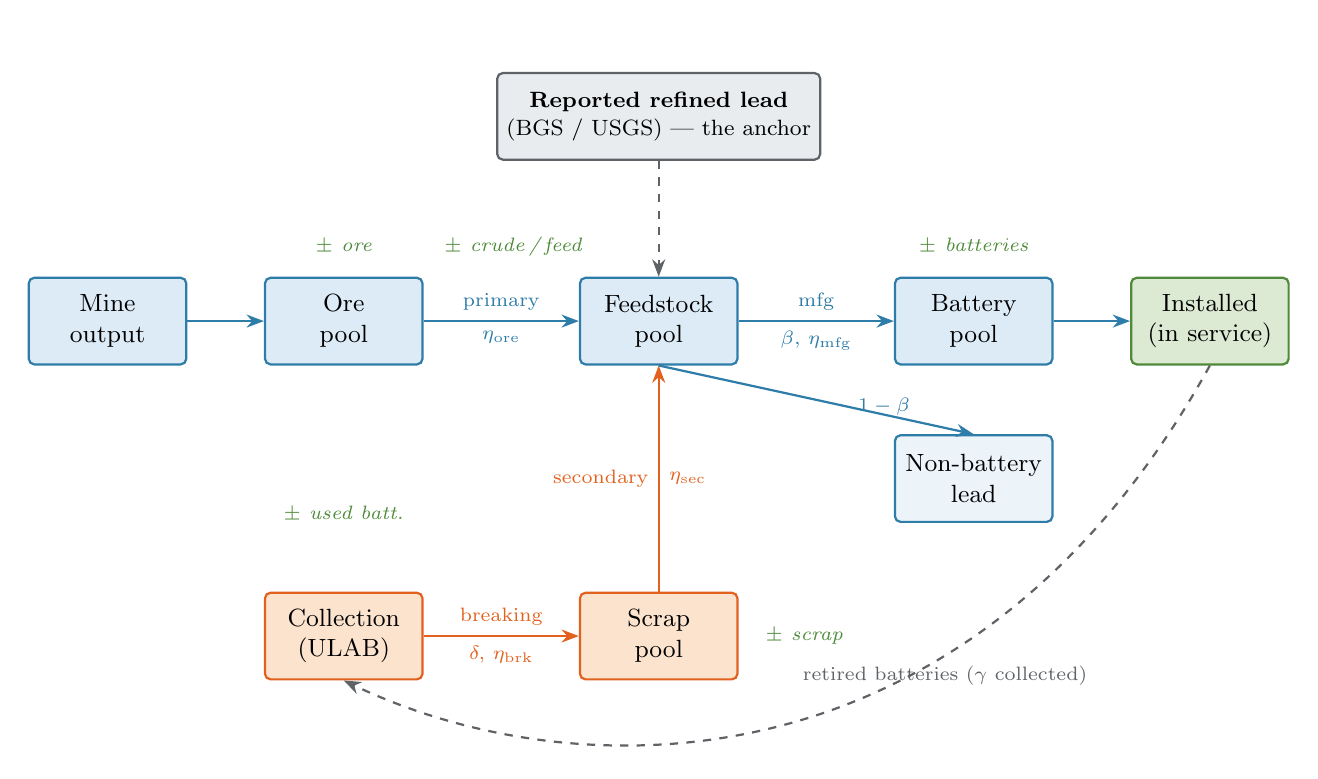
\begin{tikzpicture}[
  font=\small,
  >={Stealth[length=2.2mm]},
  pool/.style={rectangle, rounded corners=2pt, draw=headblue, fill=prodfill,
               minimum width=20mm, minimum height=11mm, align=center, thick},
  recyc/.style={rectangle, rounded corners=2pt, draw=openorange, fill=recycfill,
                minimum width=20mm, minimum height=11mm, align=center, thick},
  fin/.style={rectangle, rounded corners=2pt, draw=greenline, fill=greenfill,
              minimum width=20mm, minimum height=11mm, align=center, thick},
  anc/.style={rectangle, rounded corners=2pt, draw=pbgrey, fill=anchorfill,
              minimum width=36mm, minimum height=11mm, align=center, thick},
  tradehint/.style={greenline, font=\scriptsize\itshape},
  flow/.style={->, thick, headblue},
  rflow/.style={->, thick, openorange},
  dashflow/.style={->, thick, dashed, pbgrey},
]

% --- Forward (top) row: production, solved forward ---
\node[pool] (mine) at (0,2.4) {Mine\\output};
\node[pool] (ore)  at (3,2.4) {Ore\\pool};
\node[pool] (feed) at (7,2.4) {Feedstock\\pool};
\node[pool] (batt) at (11,2.4) {Battery\\pool};
\node[fin]  (inst) at (14,2.4) {Installed\\(in service)};

% --- Recycling (bottom) row: solved backward ---
\node[recyc] (col)   at (3,-1.6) {Collection\\(ULAB)};
\node[recyc] (scrap) at (7,-1.6) {Scrap\\pool};

% --- Non-battery branch ---
\node[pool, fill=prodfill!55] (nonb) at (11,0.4) {Non-battery\\lead};

% --- Anchor callout (top centre) ---
\node[anc] (anchor) at (7,5.0) {\footnotesize\textbf{Reported refined lead}\\[-1pt]\footnotesize (BGS / USGS) --- the anchor};
\draw[dashflow] (anchor.south) -- (feed.north);

% --- Forward arrows (blue) ---
\draw[flow] (mine) -- (ore);
\draw[flow] (ore)  -- node[above,font=\scriptsize]{primary}node[below,font=\scriptsize]{$\eta_{\mathrm{ore}}$} (feed);
\draw[flow] (feed) -- node[above,font=\scriptsize]{mfg}node[below,font=\scriptsize]{$\beta,\,\eta_{\mathrm{mfg}}$} (batt);
\draw[flow] (batt) -- (inst);
\draw[flow] (feed.south) -- node[right,font=\scriptsize,pos=0.6]{$1-\beta$} (nonb.north);

% --- Recycling arrows (orange) ---
\draw[rflow] (col)   -- node[above,font=\scriptsize]{breaking}node[below,font=\scriptsize]{$\delta,\,\eta_{\mathrm{brk}}$} (scrap);
\draw[rflow] (scrap) -- node[left,font=\scriptsize,pos=0.5]{secondary}node[right,font=\scriptsize,pos=0.5]{$\eta_{\mathrm{sec}}$} (feed);

% --- Retirement loop (installed -> collection), dashed ---
\draw[dashflow] (inst.south) .. controls (11,-3.6) and (6,-3.6) ..
  node[below,font=\scriptsize,pos=0.32]{retired batteries ($\gamma$ collected)} (col.south);

% --- Trade hints (green italic, clearly separated) ---
\node[tradehint] at (3.0,3.35)  {$\pm$ ore};
\node[tradehint] at (5.15,3.35) {$\pm$ crude\,/\,feed};
\node[tradehint] at (11.0,3.35) {$\pm$ batteries};
\node[tradehint] at (3.0,-0.05) {$\pm$ used batt.};
\node[tradehint] at (8.85,-1.6) {$\pm$ scrap};

\end{tikzpicture}

\vspace{0.9cm}
\noindent\hfill\begin{minipage}{0.92\textwidth}
\centering\footnotesize
\textcolor{headblue}{\rule[0.35ex]{2.4em}{1.2pt}}~production, solved \emph{forward} (Eq.\ 7--10)
\quad\textcolor{openorange}{\rule[0.35ex]{2.4em}{1.2pt}}~recycling, solved \emph{backward} (Eq.\ 4--6)
\quad\textcolor{pbgrey}{\rule[0.35ex]{2.4em}{1.2pt}}~anchor \& retirement loop
\quad\textcolor{greenline}{$\pm$}~trade
\end{minipage}\hfill\mbox{}

\vspace{0.8cm}
\noindent\begin{minipage}{0.9\textwidth}
\footnotesize\color{pbgrey}
The model pins the chain to reported refined-lead output (grey), then solves the
recycling stages backward (orange) and the production stages forward (blue) from that
anchor. Trade adjusts each pool ($\pm$). There is no time lag: the retired-battery loop
(dashed) is treated as steady state within a single year or multi-year average.
\end{minipage}
\end{figure}

\end{document}
